\documentclass[11pt]{article}
\usepackage[margin=1in]{geometry}
\usepackage{amsmath,amssymb}
\usepackage{booktabs}
\usepackage{graphicx}
\usepackage{xcolor}
\usepackage{tikz}
\usetikzlibrary{arrows.meta,positioning,calc}
\usepackage[hidelinks]{hyperref}
\usepackage{caption}
\usepackage{parskip}
\usepackage{float}
\usepackage{tabularx}
\usepackage{listings}
\definecolor{ink2}{HTML}{52514e}
\definecolor{cbase}{HTML}{2a78d6}
\definecolor{cone}{HTML}{eb6834}
\definecolor{ctwo}{HTML}{1baf7a}
\definecolor{cthree}{HTML}{c98500}
\definecolor{cfive}{HTML}{008300}
\definecolor{okfill}{HTML}{e8f1fb}
\definecolor{badfill}{HTML}{fdecea}
\lstset{language=Python, basicstyle=\ttfamily\scriptsize, columns=fullflexible, keepspaces=true,
  frame=single, rulecolor=\color{black!25}, backgroundcolor=\color{black!3}, commentstyle=\color{ink2}\itshape,
  keywordstyle=\color{cbase}\bfseries, showstringspaces=false, breaklines=true, aboveskip=4pt, belowskip=6pt,
  upquote=true}

\newcommand{\Unigram}{7.591}
\newcommand{\FinalThree}{3.620}
\newcommand{\FinalBaseB}{3.405}
\newcommand{\FinalAppThree}{3.376}
\newcommand{\GapBase}{0.215}
\newcommand{\GapAppThree}{0.244}
\newcommand{\CollapsedVal}{7.54}
\newcommand{\ParamsThree}{117{,}978{,}624}
\newcommand{\ParamsBase}{124{,}475{,}904}
\newcommand{\ProbePlain}{0.148}
\newcommand{\ProbeBase}{0.713}
\newcommand{\ProbeDiagEight}{0.846}
\newcommand{\ProbeMimetic}{0.956}
\newcommand{\SelfInitEight}{0.84}
\newcommand{\SelfHeadsThree}{94}
\newcommand{\SelfHeadsBase}{14}
\newcommand{\SelfHeadsAppThree}{1}
\newcommand{\SelfMeanThree}{0.61}
\newcommand{\SelfMeanBase}{0.16}
\newcommand{\SelfMeanAppThree}{0.08}
\newcommand{\RankThree}{0.873}
\newcommand{\RankCollapsed}{0.060}
\newcommand{\ShortPlain}{7.58}
\newcommand{\ShortMimetic}{6.25}
\newcommand{\ShortLearn}{5.94}
\newcommand{\ShortAnneal}{5.91}
\newcommand{\ShortAppThree}{5.86}
\newcommand{\ShortBaseB}{5.82}
\newcommand{\ValThreeAtOneK}{4.64}
\newcommand{\ValThreeAtOneTwoFiveK}{4.40}
\newcommand{\TokThree}{221}
\newcommand{\TokAppThree}{332}


\newcommand{\code}[1]{\texttt{#1}}
\newcommand{\cat}{\mathrm{Concat}_h}
\newcommand{\tr}{three\_residual}

\title{The three-residual attention block, trained with an annealed diagonal bias:\\
structure, initialization, pretraining and attention}
\author{Experiment log, branch \code{attention-experiments}}
\date{2026-10-19}

\begin{document}
\maketitle

\section*{Summary}
The \emph{\tr} block puts a residual connection on each of the three matrices of an attention head: the
attention matrix $A_h$, the value matrix $W_{vh}$ and the output matrix $W_O$. Trained from scratch on
OpenWebText as written, it collapses: within 100 steps the loss stops at the unigram level
(\CollapsedVal{} vs.\ \Unigram{}) and never moves. The collapse is already visible at initialization, where the
residual stream is nearly rank 1 by layer 11 (distance from rank 1: \ProbePlain{}; standard GPT-2: \ProbeBase{}).

Adding a bias $b=8$ to every head's self logit at initialization, then lowering it linearly to 0 over the first
1000 steps, fixes this. From step 1000 on the model is exactly \tr{} again, and it keeps training:

\begin{figure}[H]
\centering
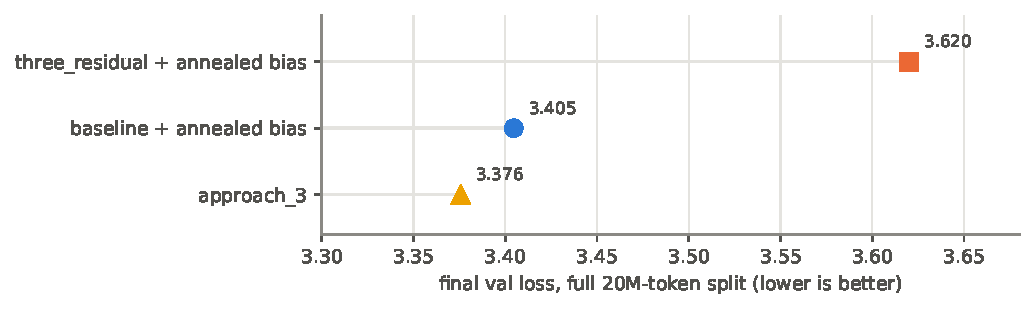
\includegraphics[width=0.78\linewidth]{figures/fig_final_loss.pdf}
\caption{Final validation loss after 2.5B OpenWebText tokens, on the full 20M-token validation split. The
\emph{baseline + annealed bias} control is standard GPT-2 trained with the same bias schedule.}
\label{fig:final}
\end{figure}

\begin{itemize}
\item \textbf{The collapse was a bad starting point, not something the block cannot learn.} With the
annealed bias, \tr{} reaches \FinalThree{}, compared with \FinalBaseB{} for the control. The gap,
\GapBase{} nats, comes from the block, since both runs used the same bias schedule.
\item \textbf{The trained \tr{} mostly attends to the token itself.} The bias is 0 for the last 3768 steps, yet
\SelfHeadsThree{} of 144 heads put more than half their weight on the token itself (control:
\SelfHeadsBase{}). With no small-scale skip path around the attention term, the model keeps each token's
state by making $A_h$ close to the identity.
\end{itemize}

\section{Setup}
\begin{center}\small
\begin{tabularx}{\linewidth}{lX}
\toprule
Data & OpenWebText, 24 of its 80 parquet shards spread evenly; GPT-2 BPE \\
 & train 2.69B tokens; validation 20M tokens (the end of the prepared stream) \\
Budget & 2.5B tokens (Chinchilla, $\approx 20$ per parameter): 4768 steps $\times$ 524{,}288 tokens \\
Optimizer & AdamW, $\beta=(0.9, 0.95)$, weight decay 0.1 (matrices only), gradient clip 1.0 \\
Learning rate & linear warmup over 250 steps to $6\times10^{-4}$, cosine decay to $6\times10^{-5}$ \\
Batch & 16 micro-batches of $32\times1024$ tokens, accumulated; bf16 autocast; one H100 GPU per run \\
Seed and order & seed 1337 and the same sequential data order in every run \\
Evaluation & 4M validation tokens every 250 steps; the full 20M tokens at the end \\
\bottomrule
\end{tabularx}
\end{center}
All losses in this report are on the same OpenWebText validation split, so they are comparable with each
other. They are \emph{not} comparable with the FineWeb-Edu numbers of the 2026-10-15/16 reports. The unigram
model (token frequencies only, no context) scores \Unigram{} on this split.

\section{Structure}
\subsection{The block}
For head $h$ (12 heads, $d = D/H = 64$), let $X_h$ be the head's $d$-dimensional slice of the raw residual stream
$X$ (before $\mathrm{LN}_1$), and $A_h$ its causal attention matrix, computed from $\mathrm{LN}_1(X)$:
\begin{align}
A_h &= \mathrm{softmax}\!\Big(\tfrac{1}{\sqrt d}\,Q_hK_h^\top + b\,I + \text{mask}\Big)
  && Q_h, K_h \text{ from } \mathrm{LN}_1(X) \\
Z_h &= A_h X_h + X_h && \text{residual on } A_h \label{eq:z}\\
Y &= \cat\big[\,Z_h W_{vh} + Z_h\,\big] && \text{residual on } W_{vh} \\
X' &= Y W_O + b_O + Y && \text{residual on } W_O \\
X^{(\ell+1)} &= X' + \mathrm{MLP}(\mathrm{LN}_2(X')) && \text{standard MLP sublayer}
\end{align}
The bias $b$ exists only during pretraining (Section~\ref{sec:init}); with $b=0$ these equations are exactly the
block in \code{src/model.py} (\code{three\_residual=True}). $W_{vh}$ is a separate $64\times64$ matrix per head,
so the value weights are block-diagonal ($12\times64\times64 = 49$k parameters, against 590k for GPT-2's full
$W_V$), and $\mathrm{LN}_1$ only feeds $Q$ and $K$. The model has \ParamsThree{} parameters
(GPT-2: \ParamsBase{}).

\begin{figure}[H]
\centering
\scalebox{0.82}{%
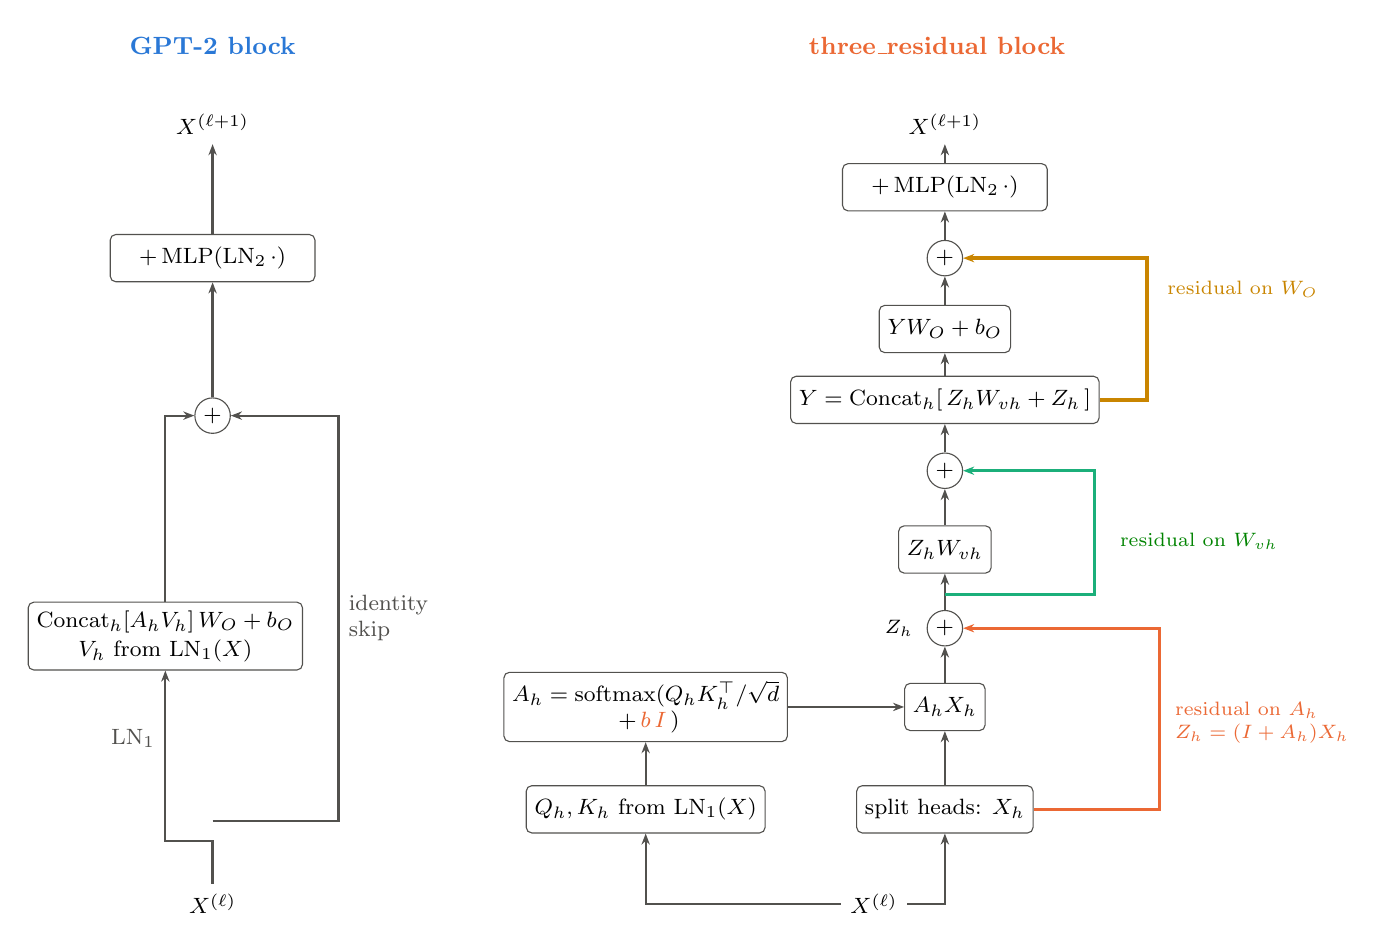
\begin{tikzpicture}[
  font=\footnotesize,
  box/.style={draw=ink2, rounded corners=2pt, minimum height=0.6cm, align=center, fill=white, inner sep=3pt},
  op/.style={draw=ink2, circle, inner sep=0.5pt, minimum size=0.45cm, fill=white},
  arr/.style={-{Stealth[length=4pt]}, ink2, thick},
  skA/.style={-{Stealth[length=4pt]}, cone, very thick},
  skV/.style={-{Stealth[length=4pt]}, ctwo, very thick},
  skO/.style={-{Stealth[length=4pt]}, cthree, very thick},
]
% ---------- left: GPT-2 ----------
\begin{scope}[shift={(-8.4,0)}]
  \node[font=\small\bfseries, text=cbase] at (0,10.9) {GPT-2 block};
  \node (x) at (0,0) {$X^{(\ell)}$};
  \node[box, minimum width=3.2cm] (att) at (-0.6,3.4) {$\cat[A_hV_h]\,W_O + b_O$\\[1pt]$V_h$ from $\mathrm{LN}_1(X)$};
  \node[op] (add) at (0,6.2) {$+$};
  \node[box, minimum width=2.6cm] (mlp) at (0,8.2) {$+\,\mathrm{MLP}(\mathrm{LN}_2\,\cdot)$};
  \node (out) at (0,9.9) {$X^{(\ell+1)}$};
  \draw[arr] (x) -- ++(0,0.8) -| node[pos=0.8, left] {$\mathrm{LN}_1$} (att.south);
  \draw[arr] (att.north) |- (add.west);
  \draw[arr] (x.north) ++(0,0.8) -- ++(1.6,0) |- node[pos=0.25, right, align=left] {identity\\skip} (add.east);
  \draw[arr] (add) -- (mlp); \draw[arr] (mlp) -- (out);
\end{scope}
% ---------- right: three_residual ----------
\node[font=\small\bfseries, text=cone] at (0.8,10.9) {three\_residual block};
\node (x) at (0,0) {$X^{(\ell)}$};
\node[box] (ln) at (-2.9,1.2) {$Q_h, K_h$ from $\mathrm{LN}_1(X)$};
\node[box] (A) at (-2.9,2.5) {$A_h=\mathrm{softmax}(Q_hK_h^\top/\sqrt d$\\$\;+\,\textcolor{cone}{b\,I}\,)$};
\node[box] (xh) at (0.9,1.2) {split heads: $X_h$};
\node[box] (ax) at (0.9,2.5) {$A_h X_h$};
\node[op] (a1) at (0.9,3.5) {$+$};
\node[left=0.05 of a1, font=\scriptsize] {$Z_h$};
\node[box] (wv) at (0.9,4.5) {$Z_h W_{vh}$};
\node[op] (a2) at (0.9,5.5) {$+$};
\node[box] (cat) at (0.9,6.4) {$Y=\cat[\,Z_hW_{vh}+Z_h\,]$};
\node[box] (wo) at (0.9,7.3) {$Y W_O + b_O$};
\node[op] (a3) at (0.9,8.2) {$+$};
\node[box, minimum width=2.6cm] (mlp) at (0.9,9.1) {$+\,\mathrm{MLP}(\mathrm{LN}_2\,\cdot)$};
\node (out) at (0.9,9.9) {$X^{(\ell+1)}$};
\draw[arr] (x) -| (ln.south);
\draw[arr] (x) -| (xh.south);
\draw[arr] (ln) -- (A);
\draw[arr] (A) -- (ax);
\draw[arr] (xh) -- (ax);
\draw[arr] (ax) -- (a1);
\draw[skA] (xh.east) -- ++(1.6,0) |- (a1.east);
\draw[arr] (a1) -- (wv);
\draw[skV] (a1.north) ++(0,0.2) -- ++(1.9,0) |- (a2.east);
\draw[arr] (wv) -- (a2);
\draw[arr] (a2) -- (cat);
\draw[arr] (cat) -- (wo);
\draw[skO] (cat.east) -- ++(0.6,0) |- (a3.east);
\draw[arr] (wo) -- (a3);
\draw[arr] (a3) -- (mlp); \draw[arr] (mlp) -- (out);
\node[font=\scriptsize, text=cone, align=left, anchor=west] at (3.7,2.3) {residual on $A_h$\\$Z_h = (I + A_h)X_h$};
\node[font=\scriptsize, text=cfive, align=left, anchor=west] at (3.0,4.6) {residual on $W_{vh}$};
\node[font=\scriptsize, text=cthree, align=left, anchor=west] at (3.6,7.8) {residual on $W_O$};
\end{tikzpicture}}
\caption{Left: the GPT-2 attention sublayer, an attention term plus an identity skip. Right: \tr{}. There is no
skip around the whole sublayer; instead each of the three matrices gets its own residual (colored arrows).
The bias $b\,I$ on the self logit (orange) is used only during pretraining and is 0 in the final model.}
\label{fig:arch}
\end{figure}

\subsection{What the three residuals do at initialization}
Ignoring LayerNorm and biases, one head's output is $(I + A_h)\,X_h\,(I + W_{vh})$, followed by $(I + W_O)$.
$W_{vh}$ and $W_O$ start small (standard deviation 0.02 and $0.02/\sqrt{24}$), so at initialization the block
computes, per head,
\[
X'_h \;\approx\; (I + A_h)\,X_h = X_h + A_h X_h .
\]
The token's own state $X_h$ is still there, but the averaged term $A_hX_h$ enters at the \emph{same} scale.
That is the difference from the variants that trained in the earlier reports: in approach\_3 the attention
term is multiplied by a small $W_O$, so the stream starts out as almost pure $X$. The residuals on $W_{vh}$ and
$W_O$ cannot help here. They act within each token's vector, while the averaging happens across tokens.

At initialization the attention is close to uniform (Figure~\ref{fig:initattn}, top row), so $A_hX_h$ is roughly
the mean of the earlier tokens. Each layer then replaces half of every token's state with that common mean.
After 12 layers, the part of the stream that has never been averaged is about $2^{-12}$ of the whole, so all
positions look nearly alike. That is the rank collapse measured in Section~\ref{sec:init}.

\section{Initialization}\label{sec:init}
\subsection{The collapse probe}
For a batch of 8 validation sequences, the probe runs the freshly initialized model and records, after every
layer, the \emph{distance from rank 1} of the residual stream:
$\lVert X - \bar X \rVert / \lVert X \rVert$, where $\bar X$ repeats the mean over positions (first 64
positions skipped). The value is 0 when every position holds the same vector. In the 2026-10-16 report, a
layer-11 value of about 0.15 or less predicted collapse in every case. The plain \tr{} sits at
\ProbePlain{}.

\subsection{Two fixes: a diagonal bias and mimetic initialization}
\textbf{Diagonal bias.} Add $b$ to each head's self logit, $\mathrm{softmax}(QK^\top/\sqrt d + b\,I)$. At
initialization the logits are close to 0, so query $i$ gives itself weight about $e^b/(e^b + i - 1)$. To
dominate around 1000 earlier positions, $e^b$ must be well above 1000, so $b \gtrsim 7$. At $b=8$ the measured
self-weight at initialization is \SelfInitEight{}; at $b=3$ and $b=5$ it is only 0.05 and 0.26, which is not
enough (Figure~\ref{fig:probe}a).

\textbf{Mimetic initialization} (after Trockman \& Kolter, 2023). Set $W_Q = W_K = s\cdot R$, with $R$ a random
orthogonal matrix. Every query then matches its own key best, with no extra parameter. Of the values tried,
only $s=1.5$ passes (Figure~\ref{fig:probe}b).

\begin{figure}[H]
\centering
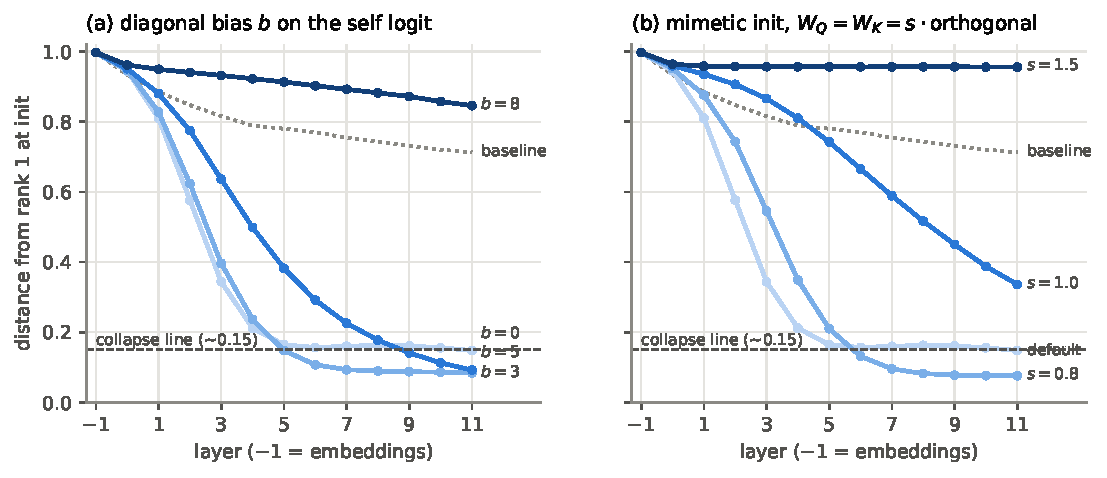
\includegraphics[width=\linewidth]{figures/fig_init_probe.pdf}
\caption{Distance from rank 1 of the residual stream after each layer, at initialization (8 validation
sequences). The dotted gray line is standard GPT-2 at initialization. Plain \tr{} ($b=0$) falls below the
collapse line by layer 5. Only $b=8$ (layer 11: \ProbeDiagEight{}) and $s=1.5$ (\ProbeMimetic{}) stay healthy.
Curiously, $b=3$ and $b=5$ end even lower than $b=0$.}
\label{fig:probe}
\end{figure}

\begin{figure}[H]
\centering
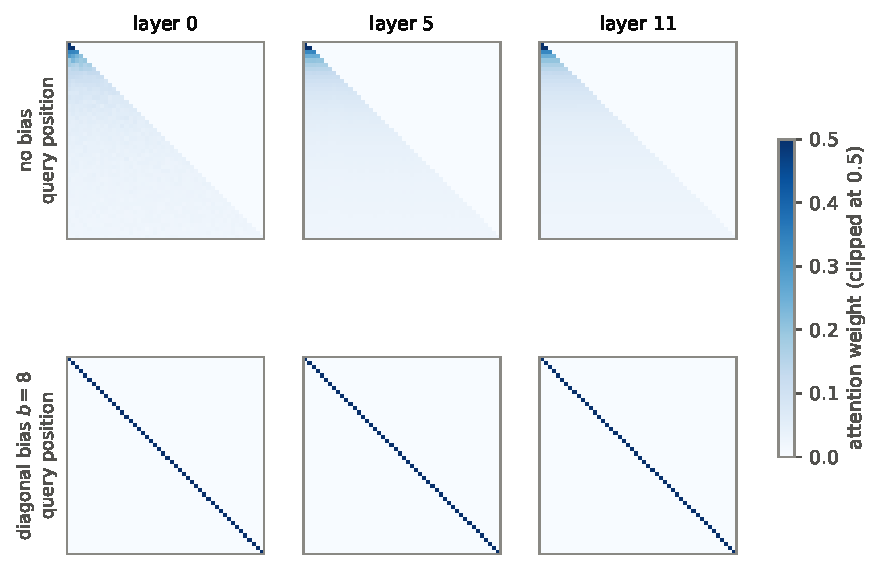
\includegraphics[width=0.74\linewidth]{figures/fig_init_attention.pdf}
\caption{Attention at initialization, averaged over the 12 heads, for the first 48 tokens of one validation
sequence. Without the bias every layer averages uniformly over the prefix (the triangle fades as rows get
longer). With $b=8$ each token attends almost only to itself, so $(I+A_h)X_h \approx 2X_h$ and nothing is
averaged away.}
\label{fig:initattn}
\end{figure}

\subsection{Short runs: which fix trains}
Each setting that passed the probe was trained for 250 steps (131M tokens), with the same schedule as a
full run:
\begin{figure}[H]
\centering
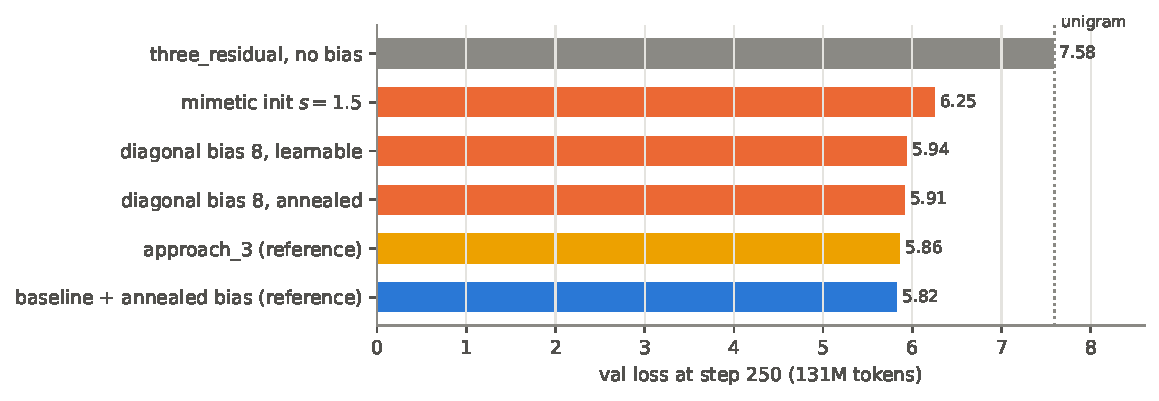
\includegraphics[width=0.8\linewidth]{figures/fig_short_runs.pdf}
\caption{Validation loss at step 250. All three fixes escape the collapse. The two diagonal-bias settings are
close to the healthy references; mimetic initialization lags, probably because its attention starts almost
entirely on the token itself (self-weight 0.99) and takes longer to spread out.}
\label{fig:short}
\end{figure}
The \emph{annealed} bias was chosen for the full run. The learnable bias trains just as well, but it would leave
an extra parameter in the final model. With annealing, the final model is exactly the \tr{} block.

\section{Pretraining}
\subsection{Bias schedule}
The bias is a non-learned buffer, set before every optimizer step $t$ to
\[
b(t) = 8\,\max\!\big(0,\; 1 - t/1000\big).
\]
It reaches exactly 0 at step 1000 and stays there, so the last 3768 steps (79\% of training) train the plain
\tr{} block. Everything else (data, order, seed, optimizer, learning rate) is identical to the other runs.

As a control, standard GPT-2 was trained with the same schedule (\emph{baseline + annealed bias}). Comparing
the two separates the cost of the block from any cost of the bias schedule. A plain GPT-2 baseline on
OpenWebText has not been run yet.

\subsection{Training curves}
\begin{figure}[H]
\centering
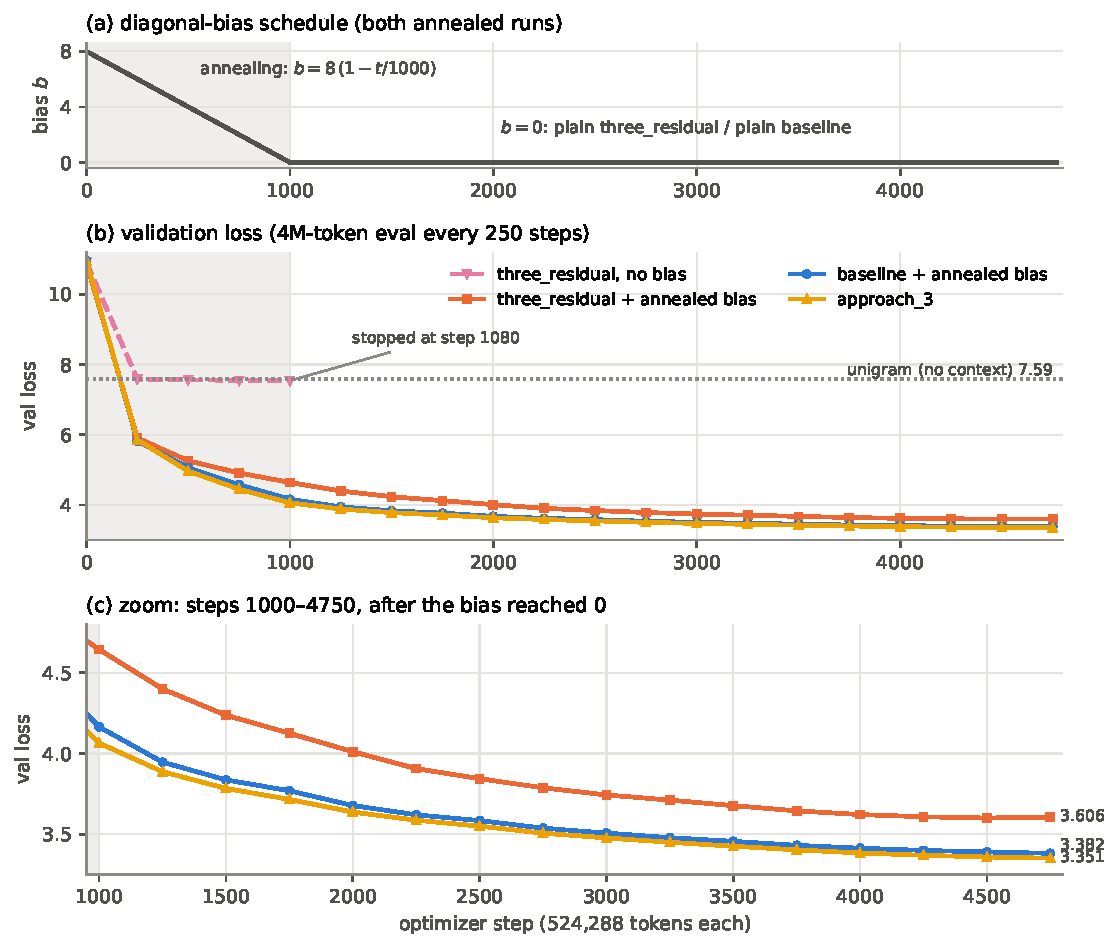
\includegraphics[width=0.94\linewidth]{figures/fig_training.pdf}
\caption{(a) Bias schedule; the shaded band marks steps 0--1000, while the bias is non-zero. (b) Validation
loss. Plain \tr{} stops at the unigram level within the first 250 steps; it was stopped at step 1080. With the
annealed bias, \tr{} follows the healthy runs during annealing and keeps improving after the bias reaches 0.
(c) Zoom on steps 1000--4750: the gap to the control narrows from 0.48 nats at step 1000 to about 0.22.}
\label{fig:training}
\end{figure}

\begin{itemize}
\item \textbf{No relapse when the bias reaches 0.} Validation loss is \ValThreeAtOneK{} at step 1000 (bias 0)
and \ValThreeAtOneTwoFiveK{} at step 1250.
\item \textbf{The gap to the control shrinks but does not close.} It falls from 0.48 nats at step 1000 to about
0.22 at the end, and it has hardly changed over the last 1000 steps.
\item \textbf{Throughput.} The bias needs an additive attention mask, which rules out PyTorch's fastest attention
kernel, so the run trained at \TokThree{}k tokens/s against \TokAppThree{}k for approach\_3 (3.1 h instead of 2 h).
The mask is kept even after the bias reaches 0. Switching back to the fast kernel at step 1000 would recover
most of that time.
\end{itemize}

\subsection{Final results}
\begin{center}\small
\begin{tabular}{lrrl}
\toprule
Model & Parameters & Final val loss & Note \\
\midrule
\tr{}, no bias & \ParamsThree{} & --- & collapsed; \CollapsedVal{} at step 1000, stopped \\
\tr{} + annealed bias & \ParamsThree{} & \FinalThree{} & bias 0 from step 1000 \\
baseline + annealed bias & \ParamsBase{} & \FinalBaseB{} & control \\
approach\_3 & \ParamsBase{} & \FinalAppThree{} & from the 2026-10-19 OpenWebText run \\
unigram & --- & \Unigram{} & token frequencies only \\
\bottomrule
\end{tabular}
\end{center}
\tr{} ends \GapBase{} nats behind the control and \GapAppThree{} behind approach\_3.

\section{Attention}
All heatmaps show the first 48 tokens of one validation sequence. All numbers (self-weight, distance from
rank 1) are averages over 8 validation sequences and query positions $\ge 64$.

\subsection{Collapsed vs.\ trained}
\begin{figure}[H]
\centering
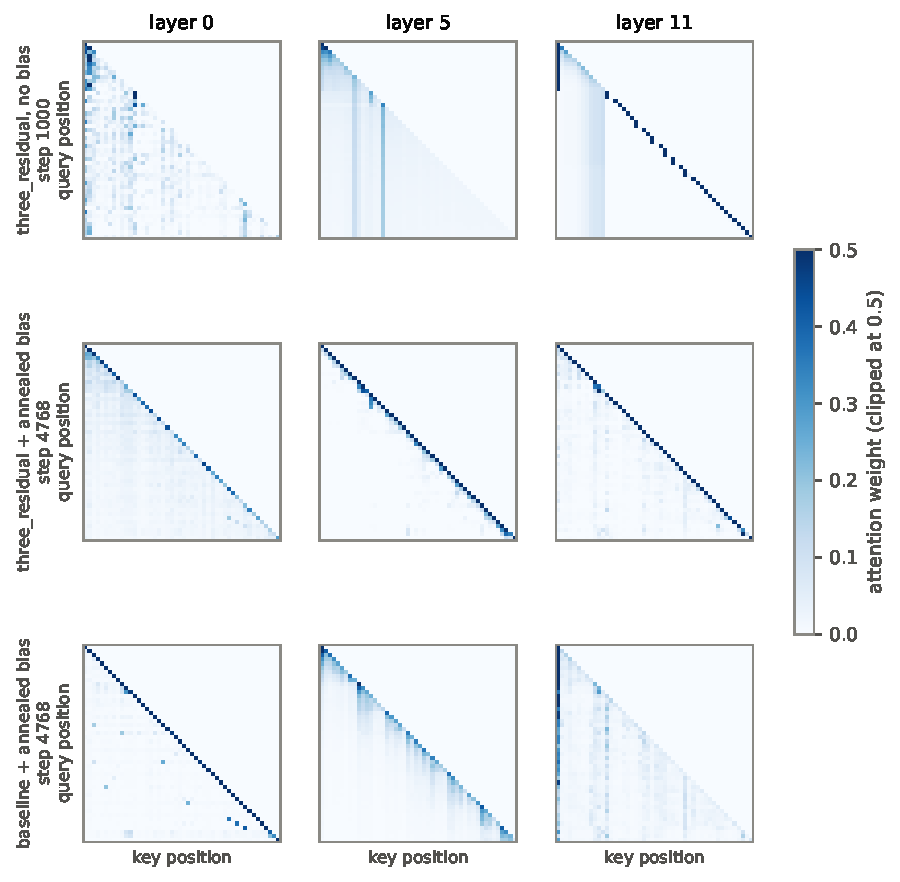
\includegraphics[width=0.78\linewidth]{figures/fig_attention_trained.pdf}
\caption{Attention averaged over heads, at layers 0, 5 and 11. Top: plain \tr{} at step 1000, after collapsing.
Middle: \tr{} trained with the annealed bias (step 4768, bias 0). Bottom: the GPT-2 control trained with the same
schedule.}
\label{fig:attn}
\end{figure}

\begin{itemize}
\item \textbf{Collapsed \tr{} (top).} Over 8 sequences its self-weight is low (at most 0.16 per layer), and many
heads read the same block of early positions. Every token gets the same output, and the residual stream ends
almost rank 1 (layer 11: \RankCollapsed{}, Figure~\ref{fig:rank}). In this one sequence, a few heads in layer
11 look sharply diagonal in the first 48 tokens; averaged over 8 sequences that pattern is weak (the token
itself is the top key in only 15--30\% of cases). An earlier quick look, based on this single sequence,
overstated it.
\item \textbf{Trained \tr{} (middle).} Strongly diagonal at every depth: each token attends mostly to itself,
with a little extra weight on nearby earlier tokens.
\item \textbf{Control (bottom).} Layer 0 is diagonal, a leftover of the bias. Deeper layers show the usual GPT-2
patterns: attention to the previous few tokens, stripes on important earlier tokens, and a column on the first
token.
\end{itemize}

\subsection{Every head of the trained \tr{}}
\begin{figure}[H]
\centering
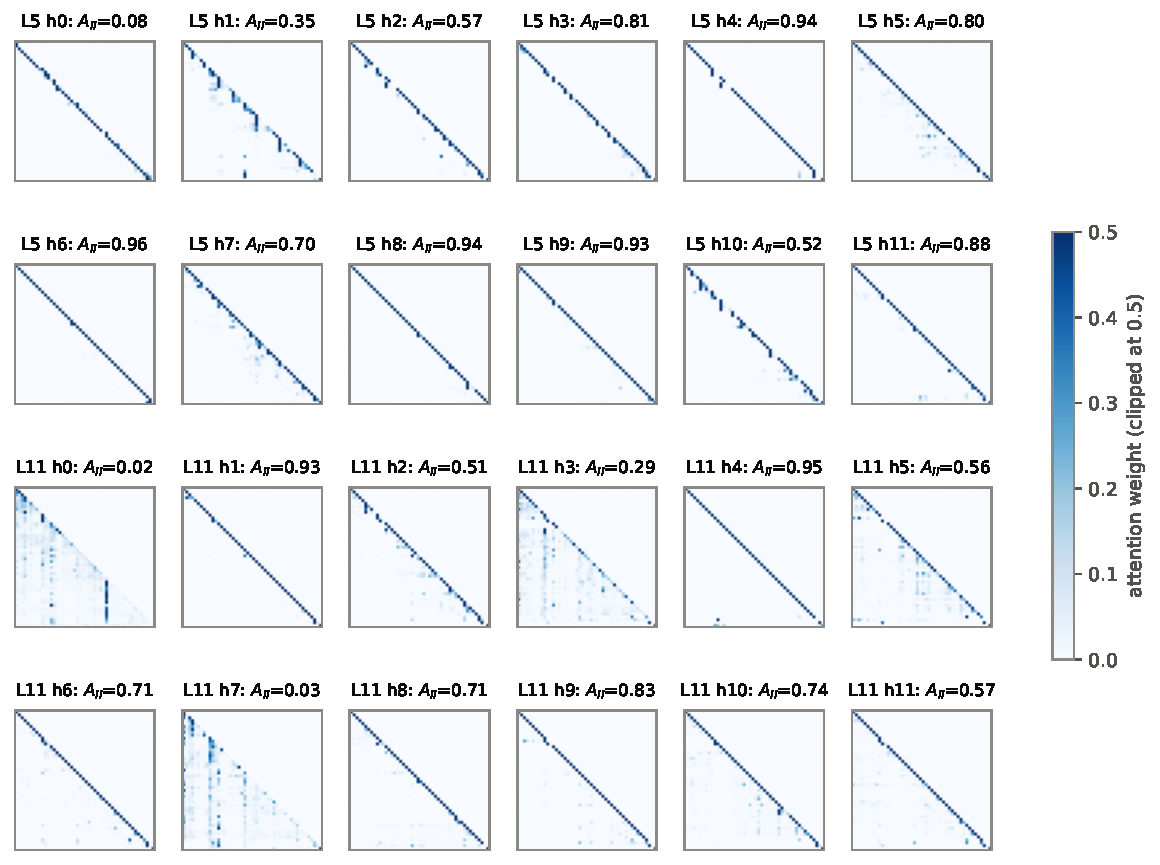
\includegraphics[width=\linewidth]{figures/fig_attention_heads.pdf}
\caption{All 12 heads of the trained \tr{} at layers 5 and 11, with each head's mean self-weight $A_{ii}$.
Most heads are almost pure self-attention. A few mix across tokens: L11 h0, h3 and h7 spread their weight over
earlier tokens, and L5 h1 and h10 attend to recent tokens. Some heads that look diagonal attend to the
\emph{previous} token, one step below the diagonal: L5 h0 looks diagonal but has $A_{ii}=0.08$.}
\label{fig:heads}
\end{figure}

\subsection{How much each head attends to itself}
\begin{figure}[H]
\centering
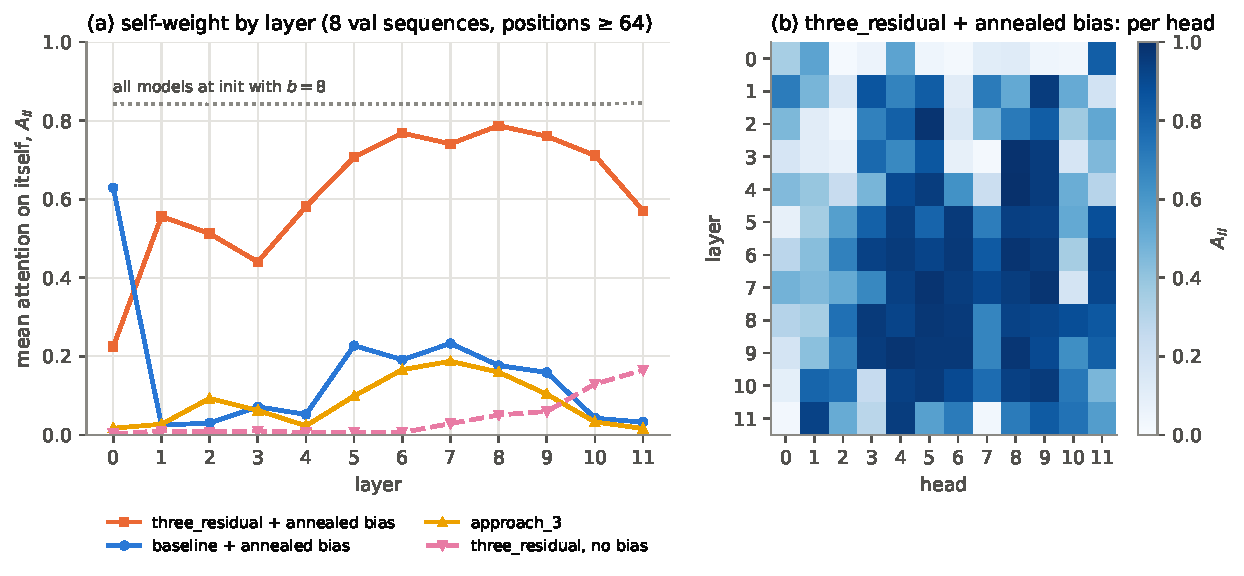
\includegraphics[width=\linewidth]{figures/fig_selfweight.pdf}
\caption{(a) Mean self-weight $A_{ii}$ per layer. All runs with the bias start at \SelfInitEight{} (dotted line).
After training, the control drops below 0.25 everywhere except layer 0, while \tr{} stays between 0.44 and 0.79
in layers 1--11. (b) Self-weight of every head in the trained \tr{}.}
\label{fig:self}
\end{figure}

\begin{center}\footnotesize
\begin{tabular}{lccc}
\toprule
 & mean $A_{ii}$ & heads with $A_{ii} > 0.5$ & weight on the 8 previous tokens \\
\midrule
\tr{} + annealed bias & \SelfMeanThree{} & \SelfHeadsThree{} / 144 & 0.21 (highest in layers 1--5) \\
baseline + annealed bias & \SelfMeanBase{} & \SelfHeadsBase{} / 144 & 0.28 (highest in layers 5--8) \\
approach\_3 & \SelfMeanAppThree{} & \SelfHeadsAppThree{} / 144 & 0.23 (highest in layers 5--8) \\
\bottomrule
\end{tabular}
\end{center}

\begin{figure}[H]
\centering
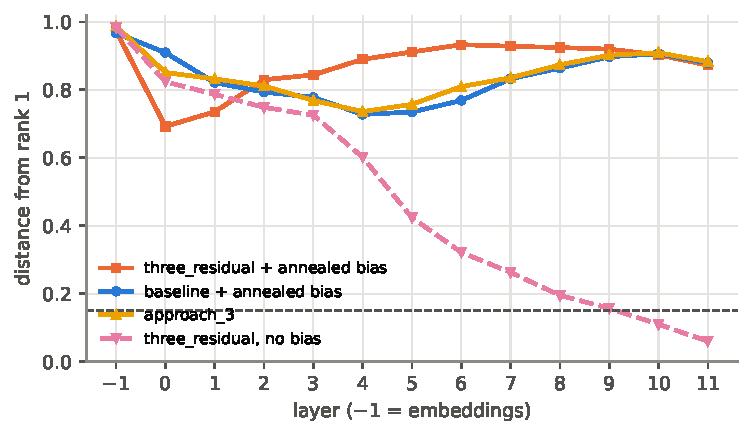
\includegraphics[width=0.62\linewidth]{figures/fig_rank_trained.pdf}
\caption{Distance from rank 1 of the residual stream in the trained models. The trained \tr{} keeps the
positions distinct (layer 11: \RankThree{}), as healthy as the control and approach\_3. The collapsed model
falls to \RankCollapsed{}.}
\label{fig:rank}
\end{figure}

\subsection{Interpretation}
The control drops its diagonal as soon as the bias is gone, because GPT-2's identity skip already carries each
token's state. \tr{} has no small-scale path of that kind: the averaged term $A_hX_h$ always enters at the
same scale as $X_h$ (Equation~\ref{eq:z}), and $W_{vh}$ and $W_O$ only act within each token. The only way it
can keep a token's own state dominant is to make $A_h$ close to $I$, and that is what most of its heads learn.

Two consequences:
\begin{itemize}
\item \textbf{Interpretability.} In \tr{}, head $h$ moves information between tokens only through
$Z_h = (I + A_h)X_h$, and the identity and the attention enter at a fixed, equal scale. So the row-normalized
matrix $\tfrac12(I + A_h)$ is head $h$'s exact token-mixing matrix on the $X$ path: it says how much of token
$i$'s new state is its own, and how much comes from each earlier token. In approach\_3 or GPT-2 this cannot be
read off $A_h$, because the attention term is rescaled by learned weights before it meets the skip.
\item \textbf{A likely cost.} Heads that are busy copying the token itself do little across tokens. In \tr{}, only
50 of 144 heads put less than half their weight on the token itself, against 130 in the control. This is a plausible reason for the
\GapBase{}-nat gap, but it has not been tested.
\end{itemize}

\section{Limitations}
\begin{itemize}
\item One seed per configuration; the seed-to-seed spread on OpenWebText has not been measured (on FineWeb-Edu it
was assumed to be about $\pm0.01$).
\item No plain GPT-2 baseline on OpenWebText yet; the control uses the same bias schedule.
\item Mimetic initialization and the learnable bias were trained for only 250 steps.
\item Heatmaps come from one sequence; the numbers in the tables are averaged over 8 sequences.
\item The collapse line (about 0.15) is an empirical rule from the earlier variants, not a derived threshold.
\end{itemize}

\section{Next steps}
\begin{enumerate}
\item Train a plain GPT-2 baseline on OpenWebText, for a clean reference.
\item Test the head-capacity explanation: for example, scale the self term, $Z_h = A_hX_h + \gamma X_h$ with a
learned $\gamma$, so heads can keep the token's state without spending their attention on it.
\item Run mimetic initialization ($s=1.5$) for the full 2.5B tokens. It needs no schedule and no extra
parameter.
\item Switch to the fast attention kernel once the bias reaches 0 (about 1.5$\times$ faster).
\end{enumerate}

\section*{Files}
\begin{tabularx}{\linewidth}{lX}
\code{code/gpt2\_torch.py} & PyTorch model used for training; variant \code{three\_residual}, options
\code{diag\_bias}, \code{diag\_learn}, \code{mimetic} \\
\code{code/model.py} & TensorFlow \code{src/model.py} with \code{three\_residual=True} \\
\code{code/three\_residual\_analysis.py} & probe, self-weight and attention maps $\rightarrow$ \code{data/} \\
\code{code/make\_three\_residual\_report.py} & figures and \code{numbers.tex} \\
\code{data/} & \code{probe\_init.json}, \code{trained.json}, \code{attention.npz}, \code{summary.json} \\
Runs & \code{/local/scratch/a/liu3170/runs/openwebtext/}: \code{tr\_diag8\_anneal1000},
\code{baseline\_diag8\_anneal1000}, \code{three\_residual} (collapsed), \code{tr\_diag8\_learn\_s250},
\code{tr\_mimetic1.5\_s250}, \code{approach\_3} \\
Command & \code{python train.py --variant three\_residual --diag\_bias 8 --anneal\_steps 1000 --data <openwebtext> --out <dir>} \\
\end{tabularx}

\appendix
\section{Code: the attention forward pass}
\begin{lstlisting}
def attend(self, q, k, v):
    if hasattr(self, 'diag'):  # diagonal bias b on the self logit (training aid)
        T = q.shape[-2]
        bias = self.causal_neg[:T, :T] + self.diag.view(-1, 1, 1) * self.eye[:T, :T]  # [H, T, T]
        return F.scaled_dot_product_attention(q, k, v, attn_mask=bias.to(q.dtype))
    return F.scaled_dot_product_attention(q, k, v, is_causal=True)

# three_residual branch of Attention.forward(x_ln, x_raw)
q, k = map(self.split_heads, self.c_attn(x_ln).split(D, dim=2))  # Q, K from LN_1(X)
xh = self.split_heads(x_raw)                                       # X_h: raw residual stream
z = self.attend(q, k, xh) + xh                                     # Z_h = A_h X_h + X_h
z = torch.einsum('bhtd,hde->bhte', z, self.w_v) + z                # Z_h W_vh + Z_h
y = z.transpose(1, 2).contiguous().view(B, T, D)                   # Y = Concat_h
return self.c_proj(y) + y                                          # Y W_O + b_O + Y

# train.py, before every optimizer step
if args.anneal_steps:
    model.set_diag(args.diag_bias * max(0.0, 1 - step / args.anneal_steps))
\end{lstlisting}

\end{document}
